\documentclass{scrartcl}

\usepackage{fixltx2e}

% Step environment
% <https://tex.stackexchange.com/a/12943/13262>
\usepackage{amsthm}
\newtheorem*{remark}{Remark}
%
\newtheoremstyle{named}{}{}{\itshape}{}{\bfseries}{.}{.5em}{\thmnote{#1 }#3}
\theoremstyle{named}
\newtheorem*{step}{Step}

\usepackage{microtype}
\usepackage{amsmath}
\usepackage{mathtools}
\usepackage{booktabs}
\usepackage{tabularx}

\usepackage{pgfplots}
\pgfplotsset{compat=newest}

\usepackage{siunitx}

\newcommand\mytitle{How to evaluate and optimize color spaces against experimental data}
\newcommand\myauthor{Nico Schlömer}

\usepackage[
  pdfencoding=unicode,
  ]{hyperref}
\hypersetup{
  pdfauthor={\myauthor},
  pdftitle={\mytitle}
}

% <https://tex.stackexchange.com/a/43009/13262>
\DeclarePairedDelimiter\abs{\lvert}{\rvert}%
\DeclarePairedDelimiter{\norm}{\lVert}{\rVert}

\usepackage[T1]{fontenc}
\usepackage{newtxtext}
\usepackage{newtxmath}

% degree symbol
\usepackage{gensymb}

% % <https://tex.stackexchange.com/a/413899/13262>
% \usepackage{etoolbox}
% \makeatletter
% \long\def\etb@listitem#1#2{%
%   \expandafter\ifblank\expandafter{\@gobble#2}
%     {}
%     {\expandafter\etb@listitem@i
%      \expandafter{\@secondoftwo#2}{#1}}}
% \long\def\etb@listitem@i#1#2{#2{#1}}
% \makeatother

% Okay. Don't use biblatex/biber for now. There are breaking changes in every
% revision, and we'd have to stick to the exact version that arxiv.org has,
% otherwise it's error messages like
% ```
% Package biblatex Warning: File 'main.bbl' is wrong format version
% - expected 2.8.
% ```
% \usepackage[sorting=none]{biblatex}
% \bibliography{bib}

\usepackage{amsmath}
\DeclareMathOperator{\sign}{sign}
\DeclareMathOperator*{\argmin}{arg\,min}

% \usepackage{amsfonts}
\usepackage{bm}
\newcommand\R{\ensuremath{\mathbb{R}}}
\newcommand\xt{\ensuremath{\bm{\tilde{x}}}}
\newcommand\yt{\ensuremath{\bm{\tilde{y}}}}

\title{\mytitle\footnote{The LaTeX sources of this article are on
\url{https://github.com/nschloe/colorio}}}
\author{\myauthor}

\begin{document}

\maketitle
\begin{abstract}
  todo
\end{abstract}

\section{Introduction}

Every year, articles on new color spaces are created, claiming that they comply to
certain experimental data better than other color spaces. In many cases, numbers are
provided in form of a table showing that the new color space is indeed better.
Unfortunately, it is hardly ever explained how those numbers are computed.

This article describes in detail how to assess the experimental compliance of color
space with experimental data. The article focuses on the two most used types of
experimental data: Hue linearity \cite{ebner,xiao,hung} and color difference ellipses
\cite{macadam1942,luorigg}.

Almost every color space is defined by a transformation $T$ that maps the CIE-1931-XYZ
coordinates into a three-dimensional new coordinate space (e.g., LAB). The
transformation is usually continuously differentiable and bijective. When talking about
a colorspace, one almost always means the transformation $T$ and its inverse.


TODO desirable properties of cost functionals:
\begin{itemize}
  \item Are continuous, and ideally continuously differentiable (for optimization)
  \item Are 0 if the experimental data is matched exactly (will never be fulfilled since
    experimental data contains errors). Together with the first one, number are small if
    the match is approximate.
  \item are scaling invariant
  \item are rotation invariant
  \item are translation invariant
\end{itemize}

% There are numerous experiments~\cite{ebner,xiao,hung,macadam,macadam,luo} which try to
% gauge perceptual distances between colors or to determine which colors of different
% luminosity are perceived as the same chroma.
%
% These experimental data have been used in the past to approximate a perceptually uniform
% colorspace, i.e., a color space in which the Euclidean distance represents the perceived
% distance, and in which colors of same chroma all sit in one line. (These two goals are
% mutually inclusive.) So far, the general approach was to assume that the transformation
% from XYZ space takes a certain mathematical form with a number of free parameters, e.g.,
% the parameters $e$, $\alpha_{i,j}$, and $\omega_{i,j}$.
% \begin{equation}\label{eq:safdar}
%   \begin{split}
%     \begin{bmatrix}
%       L\\M\\S
%     \end{bmatrix}
%     =
%     \begin{bmatrix}
%       \alpha_{1,1} & \alpha_{1,2} & 1 - \alpha_{1,1} - \alpha_{1,2}\\
%       \alpha_{2,1} & \alpha_{2,2} & 1 - \alpha_{2,1} - \alpha_{2,2}\\
%       \alpha_{3,1} & \alpha_{3,2} & 1 - \alpha_{3,1} - \alpha_{3,2}
%     \end{bmatrix}
%     \begin{bmatrix}
%       X_{D65}\\Y_{D65}\\Z_{D65}
%     \end{bmatrix}\\
%     \{L',M',S'\} = \left(\frac{c_1 + c_2\left(\frac{\{L,M,S\}}{10000}\right)^n}{1 + c_3\left(\frac{\{L,M,S\}}{10000}\right)^n}\right)^{pe}\\
%     \begin{bmatrix}
%       I_z\\a_z\\b_z
%     \end{bmatrix}
%     =
%     \begin{bmatrix}
%       \omega_{1,1} & \omega_{1,2} & 1 - \omega_{1,1} - \omega_{1,2}\\
%       \omega_{2,1} & \omega_{2,2} &   - \omega_{2,1} - \omega_{2,2}\\
%       \omega_{3,1} & \omega_{3,2} &   - \omega_{3,1} - \omega_{3,2}
%     \end{bmatrix}
%     \begin{bmatrix}
%       L'\\M'\\S'
%     \end{bmatrix}\\
%   \end{split}
% \end{equation}
% in~\cite{safdar}. Then, an optimization algorithm was applied to retrieve those
% parameters which best match the given experimental data. The resulting color space has
% then been declared ``optimal'', which held true until a new article with a different
% assumption was published which, almost by chance, achieved even better accordance with
% the data.
%
% The assumption that the transformation of XYZ to the perceptually uniform color space
% takes a particular form is of course of practical nature: A low-dimensional parameter
% space is easy to search. However, to put it mildly, it is quite optimistic to assume
% that the visual system of the brain (see figure~\ref{fig:monkey}) does a transformation that
% can be expressed in terms of some linear transformations and elementary mathematical
% functions.
%
% TODO why doesn't polynomial approximation, pade not work? runge!
%
% \begin{figure}
%   \centering
%   \includegraphics[width=0.3\textwidth]{images/monkey.png}
%   \caption{Wiring diagram of the visual system of the macaque monkey, reproduced
%   from~\cite{felleman}.}
%   \label{fig:monkey}
% \end{figure}
%
% This article describes a much more general approach and succeeds in finding a color
% space that is far more perceptually uniform that everything that has been found so far.
% Even more, there can be no color space matching the given experimental data even better.
%
% \section{Optimization problem}
%
% There are many ideas that generalize the few-parameter approaches like~\ref{eq:safdar}.
% What comes to mind are polynomial approximations
% \begin{equation}\label{eq:poly}
%   p_{\alpha}(x, y) = \sum_{i+j\le n} \alpha_{i,j} x^i y^j
% \end{equation}
% where optimization happens over the coefficients $\alpha_{i,j}$, or even fractional
% polynomials,
% \[
%   r_{\alpha, \beta}(x, y) = \frac{p_\alpha(x,y)}{q_\beta(x, y)}
% \]
% where both numerator and denominator are of the form~\ref{eq:poly} (Padé approximant).
% Both of the approaches offer the advantage that -- given an infinite source of
% experimental data -- the actual transformation $t$ can be approximated arbitrarily well
% with increased polynomial degrees. Unfortunately, polynomial approximations suffer from
% Runge's phenomenon, meaning that naively chosen reference points for the optimization
% can lead solutions which approximate $t$ well at those points, but very badly everywhere
% else. See section~\ref{sec:polyfail}.
%
% This article takes a more robust approach. The key idea is to divide the domain into
% many small triangles (see figure~\ref{fig:triangles}) and to allow each of the nodes to
% move around more or less freely such that the resulting shape matches the experimental
% data well. All continuous transformations can be approximated by this approach so it is
% reasonable to assume that we do not restrict ourselves too much here.
%
% The mathematical concept
% \[
%   F(x, y) = \begin{bmatrix}a(x,y)\\b(x,y)\end{bmatrix}
% \]
% where both $a:\Omega\to\R^2$ and $b:\Omega\to\R^2$ are piecewise linear functions on the
% triangles.
%
% Each of the two
% \[
% fl
% \]
% \[
%   \begin{split}
%   F(a_x, a_y) &=\\
%   &F_{\text{Hung--Berns}}(a_x, a_y) +
%   F_{\text{Ebner--Fairchild}}(a_x, a_y) +
%   F_{\text{Xiao}}(a_x, a_y) +\\
%   &F_{\text{MacAdam}}(a_x, a_y) +
%   F_{\text{Luo--Rigg}}(a_x, a_y) +\\
%   &F_{\Delta}(a_x, a_y)
%   \end{split}
% \]
%
% % This is achieved by dividing the xy-triangle into many smaller triangles, i.e., nodes
% % and cells, and allowing each of the nodes to move around freely to match the
% % experimental data. This is the most general approach possible; all smooth
% % transformations can be expressed in this way.
%
% TODO all cost functions must be invariant to
% \begin{itemize}
%   \item rotation,
%   \item scaling, and
%   \item translation.
% \end{itemize}

Let $(X_i, Y_i, Z_i)\in\R^3$ be a given set of points in XYZ space which, according to
some experiment, are of equal perceived hue. Consider the two non-lightness coordinates
of their image $(x_i, y_i) \coloneqq T(X_i, Y_i, Z_i)$ (see figure TODO). What is
measure of how well the points $(x_i, y_i)$ sit on a straight line? The general idea
here is to cast a line through ``the middle'' of the point cloud and sum up the
distances of all points to that line. There are multiple meaningful ways in which
``the middle'' and ``distance'' can be defined. Remember that in $\R^n$, the distance
between two points $a$ and $b$ can be defined by a \emph{norm}.


\subsection{Cost functional for target distances and ellipses}

Some data sets give target distance values $d_i$ for pairs of colors $X_{i,1}, X_{i,2}$
(e.g. \cite{macadam1974}). A color space conforms with this data if the distance
between the transformed points
$\delta_i \coloneqq \norm{T(X_{i,1}) - T(X_{i,2})}_2$
is close to a scaled $d_i$, i.e.,
\begin{equation}\label{eq:p}
  p_2
  \coloneqq \sqrt{\sum_{i=1}^n (\alpha d_i - \delta_i)^2}
\end{equation}
The parameter $\alpha$ is chosen to minimize the expression, namely, $\alpha =
\left.\sum_{i=1}^n d_i \delta_i \middle/ \sum_{i=1}^n d_i^2\right.$.
To achieve scale-invariance, one often divides by
$\sqrt{\sum_{i=1}^n \delta_i^2}$.
The resulting expression is always between 0 and 1, and after scaling by 100, this is
called the STRESS (STandardized REsidual Sum of Squares) metric for target distances,
\begin{equation}\label{eq:p}
  p_{\text{STRESS}}
  \coloneqq
  100
  \frac{%
    \sqrt{\sum_{i=1}^n (\alpha d_i - \delta_i)^2}
  }{
    \sqrt{\sum_{i=1}^n \delta_i^2}
  }.
\end{equation}

\begin{figure}
  \centering
  % This file was created by tikzplotlib vunknown.
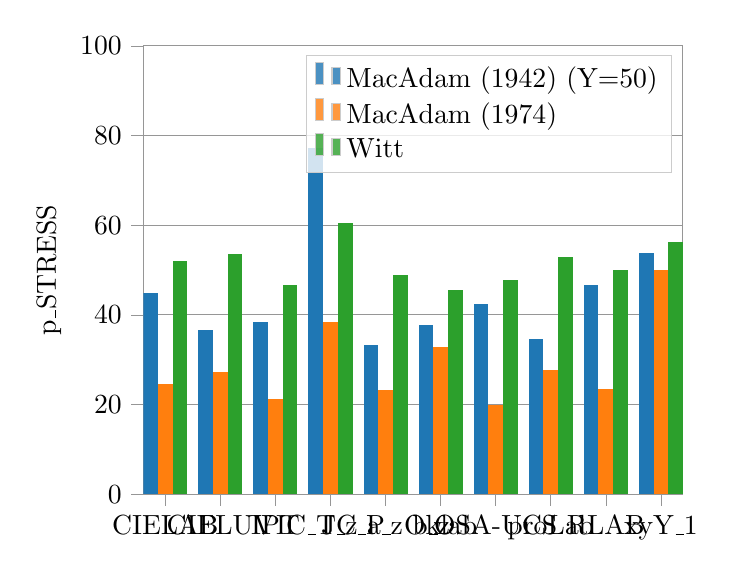
\begin{tikzpicture}

\definecolor{color0}{rgb}{0.12156862745098,0.466666666666667,0.705882352941177}
\definecolor{color1}{rgb}{1,0.498039215686275,0.0549019607843137}
\definecolor{color2}{rgb}{0.172549019607843,0.627450980392157,0.172549019607843}

\begin{axis}[
axis line style={white!58.8235294117647!black},
legend cell align={left},
legend style={fill opacity=0.8, draw opacity=1, text opacity=1, draw=white!80!black},
tick align=outside,
tick pos=left,
x grid style={white!58.8235294117647!black},
xmin=-0.4, xmax=9.4,
xtick style={color=white!58.8235294117647!black},
xtick={0,1,2,3,4,5,6,7,8,9},
xticklabels={CIELAB,CIELUV,IPT,IC\_TC\_P,J\_z a\_z b\_z,Oklab,OSA-UCS,proLab,RLAB,xyY\_1},
y grid style={white!58.8235294117647!black},
ylabel={p\_STRESS},
ymajorgrids,
ymin=0, ymax=100,
ytick style={color=white!58.8235294117647!black}
]
\draw[draw=none,fill=color0] (axis cs:-0.4,0) rectangle (axis cs:-0.133333333333333,44.8952155515788);
\addlegendimage{ybar,ybar legend,draw=none,fill=color0};
\addlegendentry{MacAdam (1942) (Y=50)}

\draw[draw=none,fill=color0] (axis cs:0.6,0) rectangle (axis cs:0.866666666666667,36.5010276032748);
\draw[draw=none,fill=color0] (axis cs:1.6,0) rectangle (axis cs:1.86666666666667,38.4833636095126);
\draw[draw=none,fill=color0] (axis cs:2.6,0) rectangle (axis cs:2.86666666666667,77.2316903365103);
\draw[draw=none,fill=color0] (axis cs:3.6,0) rectangle (axis cs:3.86666666666667,33.2757088119244);
\draw[draw=none,fill=color0] (axis cs:4.6,0) rectangle (axis cs:4.86666666666667,37.6772548200669);
\draw[draw=none,fill=color0] (axis cs:5.6,0) rectangle (axis cs:5.86666666666667,42.4396646797378);
\draw[draw=none,fill=color0] (axis cs:6.6,0) rectangle (axis cs:6.86666666666667,34.635501753967);
\draw[draw=none,fill=color0] (axis cs:7.6,0) rectangle (axis cs:7.86666666666667,46.581942046651);
\draw[draw=none,fill=color0] (axis cs:8.6,0) rectangle (axis cs:8.86666666666667,53.7506022511023);
\draw[draw=none,fill=color1] (axis cs:-0.133333333333333,0) rectangle (axis cs:0.133333333333333,24.5319191673876);
\addlegendimage{ybar,ybar legend,draw=none,fill=color1};
\addlegendentry{MacAdam (1974)}

\draw[draw=none,fill=color1] (axis cs:0.866666666666667,0) rectangle (axis cs:1.13333333333333,27.1465135470917);
\draw[draw=none,fill=color1] (axis cs:1.86666666666667,0) rectangle (axis cs:2.13333333333333,21.2696481498459);
\draw[draw=none,fill=color1] (axis cs:2.86666666666667,0) rectangle (axis cs:3.13333333333333,38.4505318024105);
\draw[draw=none,fill=color1] (axis cs:3.86666666666667,0) rectangle (axis cs:4.13333333333333,23.2111338532765);
\draw[draw=none,fill=color1] (axis cs:4.86666666666667,0) rectangle (axis cs:5.13333333333333,32.7178547285273);
\draw[draw=none,fill=color1] (axis cs:5.86666666666667,0) rectangle (axis cs:6.13333333333333,19.8475379525657);
\draw[draw=none,fill=color1] (axis cs:6.86666666666667,0) rectangle (axis cs:7.13333333333333,27.7092844635432);
\draw[draw=none,fill=color1] (axis cs:7.86666666666667,0) rectangle (axis cs:8.13333333333333,23.5028573394472);
\draw[draw=none,fill=color1] (axis cs:8.86666666666667,0) rectangle (axis cs:9.13333333333333,50.0184864244504);
\draw[draw=none,fill=color2] (axis cs:0.133333333333333,0) rectangle (axis cs:0.4,51.9845666548853);
\addlegendimage{ybar,ybar legend,draw=none,fill=color2};
\addlegendentry{Witt}

\draw[draw=none,fill=color2] (axis cs:1.13333333333333,0) rectangle (axis cs:1.4,53.5668514182667);
\draw[draw=none,fill=color2] (axis cs:2.13333333333333,0) rectangle (axis cs:2.4,46.7222778094553);
\draw[draw=none,fill=color2] (axis cs:3.13333333333333,0) rectangle (axis cs:3.4,60.5016229218686);
\draw[draw=none,fill=color2] (axis cs:4.13333333333333,0) rectangle (axis cs:4.4,48.8370743196918);
\draw[draw=none,fill=color2] (axis cs:5.13333333333333,0) rectangle (axis cs:5.4,45.4213412985957);
\draw[draw=none,fill=color2] (axis cs:6.13333333333333,0) rectangle (axis cs:6.4,47.6753713547588);
\draw[draw=none,fill=color2] (axis cs:7.13333333333333,0) rectangle (axis cs:7.4,52.78820194734);
\draw[draw=none,fill=color2] (axis cs:8.13333333333333,0) rectangle (axis cs:8.4,50.0899025149911);
\draw[draw=none,fill=color2] (axis cs:9.13333333333333,0) rectangle (axis cs:9.4,56.1591454267207);
\end{axis}

\end{tikzpicture}

  \caption{$p_\text{STRESS}$ for a number of color spaces. The color space OSA-UCS was
  designed specifically with the MacAdam \cite{macadam1974} dataset in mind. Both CAM
  spaces perform well for all data sets.}
\end{figure}

A common special case of this setting is distance data given in terms of ellipse points,
i.e., a color center with a number of standard deviations (or similar) in various
directions. The famous MacAdam ellipses (\cite{macadam1942}) are derived from such data.
Since the ellipses are supposed to to be circles of equal size in the transformed space,
the target value for all $d_i$ is 1. The parameter $\alpha$ simplifies to be the average
over all $\delta_i$ and we have
\begin{equation}\label{eq:e}
  e_{\text{STRESS}}
  \coloneqq
  100
  \frac{%
    \sqrt{\sum_{i=1}^n (\alpha - \delta_{i})^2}
  }{
    \sqrt{\sum_{i=1}^n \delta_i^2}
  }.
\end{equation}
In case only the actual ellipses are given (e.g., \cite{luorigg}), one can place a
number of points onto their boundaries (e.g., 8 or 16) and compute the residual with
from them.

\begin{table}
  \centering
  \begin{tabular}{lrr}
    \toprule
    & MacAdam & Luo-Rigg(8) \cite{luorigg}\\
    \midrule
CAM02 (UCS)   & \textbf{27.2} &         30.1\\
CAM16 (UCS)   &         29.0  & \textbf{28.4}\\
CIELAB        &         57.3  &         48.5\\
CIELUV        &         36.5  &         45.3\\
IPT           &         38.5  &         47.5\\
$IC_TC_P$     &         75.9  &         61.2\\
$J_z a_z b_z$ &         40.7  &         40.3\\
Oklab         &         37.7  &         39.1\\
OSA-UCS       &         63.6  &         42.2\\
RLAB          &         46.6  &         46.6\\
xyY           &         53.8  &         44.0\\
    \bottomrule
  \end{tabular}
  \caption{$e_\text{STRESS}$ for a number of color spaces. CAM02 and its close relative
  CAM16 far outperform the other color spaces, particularly for the Luo-Rigg data set.}
\end{table}

\subsection{Cost functional for hue linearity}

There are multiple experiments which data about which colors are perceived to be of
equal hue~\cite{hung,ebner,xiao} (see figure~\ref{}). Color spaces are considered good
if the transformation maps points of equal perceived hue onto a straight line.

What is a good measure of how well points sit on a straight line?
A common idea is to find the straight line that mimizes the sum of squared distances to
all points. This general approach is usually referred to as \emph{total least squares
(TLS)}.
The line is typically
given implicitly by $\alpha_1 x + \alpha_2 y
= 0$ with $\alpha_1,\alpha_2\in\R$, $\|\alpha\|_2^2 = \alpha_1^2 + \alpha_2^2 = 1$.
Because this assumes that the line passes through the origin, all points are
first translated such that the whitepoint sits in in origin.

For scale-invariance, it is convenient to divide by the maximizer of the squared
distances, in total:
\begin{equation}\label{eq:l}
l_2 \coloneqq
  \frac{
\min_{\|\alpha\|_2=1}
  \sqrt{\sum_{i=1}^n (\alpha_1 \tilde{x}_i + \alpha_2 \tilde{y}_i)^2}
}{
\max_{\|\alpha\|_2=1}
  \sqrt{\sum_{i=1}^n (\alpha_1 \tilde{x}_i + \alpha_2 \tilde{y}_i)^2}
}
\end{equation}
with the translated sample points
\[
  \tilde{x}_i \coloneqq x_i-w_x,\qquad
  \tilde{y}_i \coloneqq y_i-w_y.
\]

The value of $l_2$ can be approximated with any appropriate optimization method. A more
explicit and more easily computable representation however is retrieved as follows.
With the $n$-by-2 coordinate matrix
\[
  A \coloneqq \begin{pmatrix}
    \tilde{x}_1 & \tilde{y}_1\\
    \vdots & \vdots\\
    \tilde{x}_n & \tilde{y}_n
  \end{pmatrix},
\]
the sum in \eqref{eq:l} can be written as
\[
  \sum_{i=1}^n (\alpha_1 \tilde{x}_i + \alpha_2 \tilde{y}_i)^2
  = (A \alpha)^T (A \alpha)
  = \alpha^T A^T A \alpha.
\]
This makes clear that $l_2$ is exactly the ratio of the square roots of the two
eigenvalues of $A^TA$ or equivalently the ratio of the two singular values of $A$,
\[
l_2
= \frac{
  \sqrt{\lambda_{\min}(A^T A)}
  }{
    \sqrt{\lambda_{\max}(A^T A)}
  }
= \frac{\sigma_{\min}(A)}{\sigma_{\max}(A)}.
\]
The value is given explicitly by
\begin{equation*}
  l_2 = \sqrt{
    \frac{
      \xt^T\xt
      + \yt^T\yt
      - \sqrt{(\xt^T\xt - \yt^T\yt)^2 + 4 (\xt^T\yt)^2}
    }{
      \xt^T\xt
      + \yt^T\yt
      + \sqrt{(\xt^T\xt - \yt^T\yt)^2 + 4 (\xt^T\yt)^2}
    }
    }.
\end{equation*}
The expression under the outer root is indeed always nonnegative by virtue of the
Cauchy-Schwarz inequality $(\xt^T\yt)^2 \le (\xt^T\xt) (\yt^T\yt)$. It is 0 if and only
if $\xt$ and $\yt$ are linearly dependent, i.e., if the points $(x_i, y_i)$ sit on a
straight line through the origin.

Since $0\le l_2\le 1$, the value can be given in terms of STRESS,
\begin{equation}\label{eq:lstress}
  l_\text{STRESS} = 100 \frac{\sigma_{\min}(A)}{\sigma_{\max}(A)}.
\end{equation}


% \begin{remark}
%   The representation \eqref{eq:s2} is suitable for optimization purposes. Since a value
%   $\sqrt{t}$ is small if and only if $t$ is small, one would in the interest of
%   simplicity disregard the outer square root.
% \end{remark}

\begin{remark}
Besides \eqref{eq:l}, there are other meaningful ways in which the distance of a point
cloud to a line can be defined. Instead of summing the squared distances, one could take
the $p$-norm,
\[
l_p
  \coloneqq
  \frac{
    \min_{\|\alpha\|_2=1} \|\alpha_1 \tilde{x} + \alpha_2\tilde{y}\|_p
  }{
    \max_{\|\alpha\|_2=1} \|\alpha_1 \tilde{x} + \alpha_2\tilde{y}\|_p
  }
  = \frac{
    \min_{\|\alpha\|_2=1}
  \left(\sum_{i=1}^n |\alpha_1 \tilde{x}_i + \alpha_2 \tilde{y}_i|^p\right)^{1/p}
}{
    \max_{\|\alpha\|_2=1}
  \left(\sum_{i=1}^n |\alpha_1 \tilde{x}_i + \alpha_2 \tilde{y}_i|^p\right)^{1/p}
}
\]
  with $1\le p \le \infty$.
  The value $l_2$ remains of prominent importance, though, because of its smooth
  dependence on the point set.
\end{remark}


\begin{figure}
  \centering
  % This file was created by tikzplotlib vunknown.
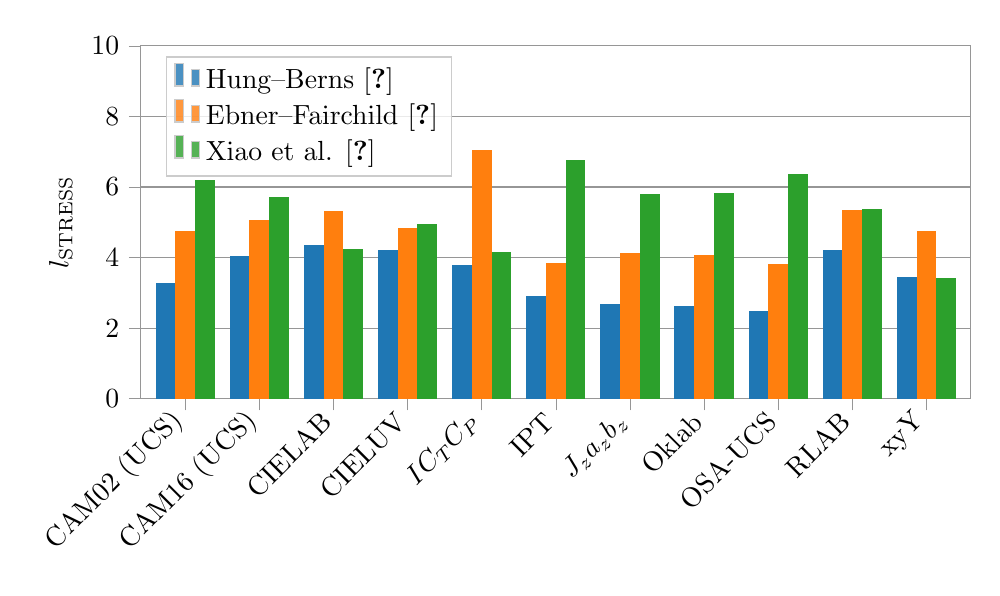
\begin{tikzpicture}

\definecolor{color0}{rgb}{0.12156862745098,0.466666666666667,0.705882352941177}
\definecolor{color1}{rgb}{1,0.498039215686275,0.0549019607843137}
\definecolor{color2}{rgb}{0.172549019607843,0.627450980392157,0.172549019607843}

\begin{axis}[
axis line style={white!58.8235294117647!black},
legend cell align={left},
width=\textwidth,
height=0.5\textwidth,
legend style={fill opacity=0.8, draw opacity=1, text opacity=1, at={(0.03,0.97)}, anchor=north west, draw=white!80!black},
tick align=outside,
tick pos=left,
x grid style={white!58.8235294117647!black},
xmin=-0.6, xmax=10.6,
xtick style={color=white!58.8235294117647!black},
xtick={0,1,2,3,4,5,6,7,8,9,10},
xticklabels={CAM02 (UCS),CAM16 (UCS),CIELAB,CIELUV,$IC_TC_P$,IPT,$J_za_zb_z$,Oklab,OSA-UCS,RLAB,xyY},
xticklabel style={rotate=45,anchor=east},
y grid style={white!58.8235294117647!black},
ylabel={$l_\text{STRESS}$},
ymajorgrids,
ymin=0, ymax=10.0,
ytick style={color=white!58.8235294117647!black}
]
\draw[draw=none,fill=color0] (axis cs:-0.4,0) rectangle (axis cs:-0.133333333333333,3.26752096358107);
\addlegendimage{ybar,ybar legend,draw=none,fill=color0};
  \addlegendentry{Hung--Berns \cite{hung}}

\draw[draw=none,fill=color0] (axis cs:0.6,0) rectangle (axis cs:0.866666666666667,4.03663610711868);
\draw[draw=none,fill=color0] (axis cs:1.6,0) rectangle (axis cs:1.86666666666667,4.34856818798823);
\draw[draw=none,fill=color0] (axis cs:2.6,0) rectangle (axis cs:2.86666666666667,4.21626028738579);
\draw[draw=none,fill=color0] (axis cs:3.6,0) rectangle (axis cs:3.86666666666667,3.7957739893557);
\draw[draw=none,fill=color0] (axis cs:4.6,0) rectangle (axis cs:4.86666666666667,2.92119683105356);
\draw[draw=none,fill=color0] (axis cs:5.6,0) rectangle (axis cs:5.86666666666667,2.68536426894407);
\draw[draw=none,fill=color0] (axis cs:6.6,0) rectangle (axis cs:6.86666666666667,2.63371950519246);
\draw[draw=none,fill=color0] (axis cs:7.6,0) rectangle (axis cs:7.86666666666667,2.49530998013144);
\draw[draw=none,fill=color0] (axis cs:8.6,0) rectangle (axis cs:8.86666666666667,4.20182174798341);
\draw[draw=none,fill=color0] (axis cs:9.6,0) rectangle (axis cs:9.86666666666667,3.44018748653443);
\draw[draw=none,fill=color1] (axis cs:-0.133333333333333,0) rectangle (axis cs:0.133333333333333,4.75235322590395);
\addlegendimage{ybar,ybar legend,draw=none,fill=color1};
  \addlegendentry{Ebner--Fairchild \cite{ebner}}

\draw[draw=none,fill=color1] (axis cs:0.866666666666667,0) rectangle (axis cs:1.13333333333333,5.07600805665883);
\draw[draw=none,fill=color1] (axis cs:1.86666666666667,0) rectangle (axis cs:2.13333333333333,5.30715095336481);
\draw[draw=none,fill=color1] (axis cs:2.86666666666667,0) rectangle (axis cs:3.13333333333333,4.82895376092783);
\draw[draw=none,fill=color1] (axis cs:3.86666666666667,0) rectangle (axis cs:4.13333333333333,7.04859738515855);
\draw[draw=none,fill=color1] (axis cs:4.86666666666667,0) rectangle (axis cs:5.13333333333333,3.8585452834895);
\draw[draw=none,fill=color1] (axis cs:5.86666666666667,0) rectangle (axis cs:6.13333333333333,4.11463844121543);
\draw[draw=none,fill=color1] (axis cs:6.86666666666667,0) rectangle (axis cs:7.13333333333333,4.05730886560147);
\draw[draw=none,fill=color1] (axis cs:7.86666666666667,0) rectangle (axis cs:8.13333333333333,3.81297237590754);
\draw[draw=none,fill=color1] (axis cs:8.86666666666667,0) rectangle (axis cs:9.13333333333333,5.35024616302759);
\draw[draw=none,fill=color1] (axis cs:9.86666666666667,0) rectangle (axis cs:10.1333333333333,4.75045818919244);
\draw[draw=none,fill=color2] (axis cs:0.133333333333333,0) rectangle (axis cs:0.4,6.20819583068419);
\addlegendimage{ybar,ybar legend,draw=none,fill=color2};
  \addlegendentry{Xiao et al. \cite{xiao}}

\draw[draw=none,fill=color2] (axis cs:1.13333333333333,0) rectangle (axis cs:1.4,5.72257615772008);
\draw[draw=none,fill=color2] (axis cs:2.13333333333333,0) rectangle (axis cs:2.4,4.23955931207367);
\draw[draw=none,fill=color2] (axis cs:3.13333333333333,0) rectangle (axis cs:3.4,4.94778942179491);
\draw[draw=none,fill=color2] (axis cs:4.13333333333333,0) rectangle (axis cs:4.4,4.1670522430841);
\draw[draw=none,fill=color2] (axis cs:5.13333333333333,0) rectangle (axis cs:5.4,6.77347388639467);
\draw[draw=none,fill=color2] (axis cs:6.13333333333333,0) rectangle (axis cs:6.4,5.79350009458213);
\draw[draw=none,fill=color2] (axis cs:7.13333333333333,0) rectangle (axis cs:7.4,5.83206308550632);
\draw[draw=none,fill=color2] (axis cs:8.13333333333333,0) rectangle (axis cs:8.4,6.37866193244541);
\draw[draw=none,fill=color2] (axis cs:9.13333333333333,0) rectangle (axis cs:9.4,5.38373889554062);
\draw[draw=none,fill=color2] (axis cs:10.1333333333333,0) rectangle (axis cs:10.4,3.40752186432328);
\end{axis}

\end{tikzpicture}

  \caption{$l_\text{STRESS}$ averaged over all arms of each data set.  While all listed
  color spaces perform quite well, OSA-UCS is the overall best color space for hue
  linearity.}
\end{figure}

\subsection{Cost functional for lightness data}

\cite{fairchildchen}

\begin{figure}
  \centering
  % This file was created by tikzplotlib v0.9.7.
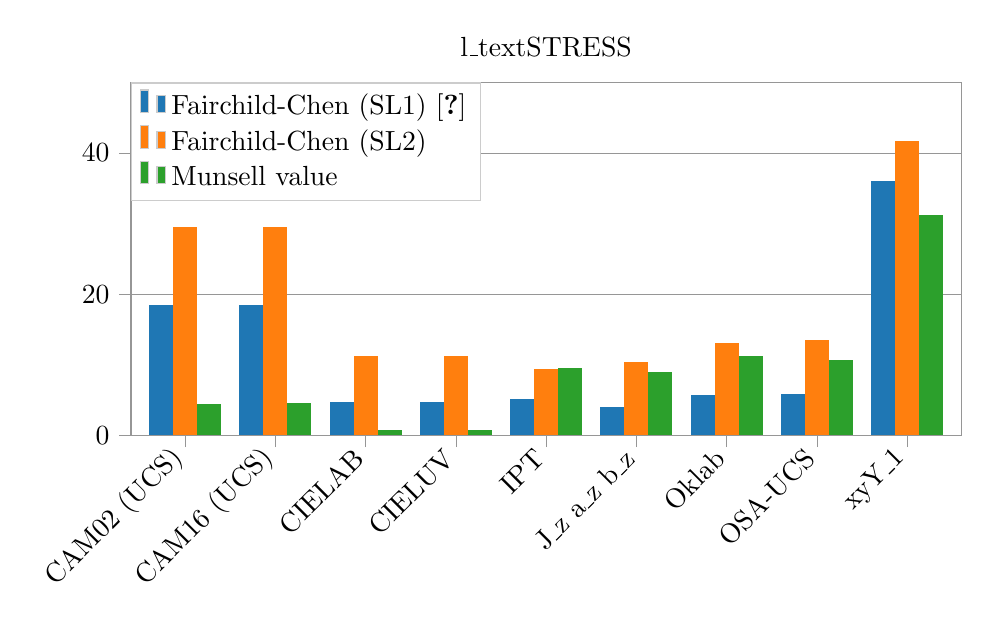
\begin{tikzpicture}

\definecolor{color0}{rgb}{0.12156862745098,0.466666666666667,0.705882352941177}
\definecolor{color1}{rgb}{1,0.498039215686275,0.0549019607843137}
\definecolor{color2}{rgb}{0.172549019607843,0.627450980392157,0.172549019607843}

\begin{axis}[
axis line style={white!58.8235294117647!black},
height=0.5\textwidth,
legend cell align={left},
legend style={
  fill opacity=1,
  draw opacity=1,
  text opacity=1,
  at={(0,1)},
  anchor=north west,
  draw=white!80!black
},
tick align=outside,
tick pos=left,
title={l\_{text{STRESS}}},
width=\textwidth,
x grid style={white!58.8235294117647!black},
xmin=-0.6, xmax=8.6,
xtick style={color=white!58.8235294117647!black},
xtick={0,1,2,3,4,5,6,7,8},
xticklabel style={rotate=45.0,anchor=east},
xticklabels={CAM02 (UCS),CAM16 (UCS),CIELAB,CIELUV,IPT,J\_z a\_z b\_z,Oklab,OSA-UCS,xyY\_1},
y grid style={white!58.8235294117647!black},
ymajorgrids,
ymin=0, ymax=50,
ytick style={color=white!58.8235294117647!black},
yticklabel style={anchor=east}
]
\draw[draw=none,fill=color0] (axis cs:-0.4,0) rectangle (axis cs:-0.133333333333333,18.4645911268359);
\addlegendimage{ybar,ybar legend,draw=none,fill=color0};
\addlegendentry{Fairchild-Chen (SL1) \cite{fairchildchen}}

\draw[draw=none,fill=color0] (axis cs:0.6,0) rectangle (axis cs:0.866666666666667,18.462147583011);
\draw[draw=none,fill=color0] (axis cs:1.6,0) rectangle (axis cs:1.86666666666667,4.67289145504149);
\draw[draw=none,fill=color0] (axis cs:2.6,0) rectangle (axis cs:2.86666666666667,4.67289145504149);
\draw[draw=none,fill=color0] (axis cs:3.6,0) rectangle (axis cs:3.86666666666667,5.16507600277125);
\draw[draw=none,fill=color0] (axis cs:4.6,0) rectangle (axis cs:4.86666666666667,4.0793287828234);
\draw[draw=none,fill=color0] (axis cs:5.6,0) rectangle (axis cs:5.86666666666667,5.64665508676546);
\draw[draw=none,fill=color0] (axis cs:6.6,0) rectangle (axis cs:6.86666666666667,5.82738652177515);
\draw[draw=none,fill=color0] (axis cs:7.6,0) rectangle (axis cs:7.86666666666667,35.9945312574285);
\draw[draw=none,fill=color1] (axis cs:-0.133333333333333,0) rectangle (axis cs:0.133333333333333,29.5046968567554);
\addlegendimage{ybar,ybar legend,draw=none,fill=color1};
\addlegendentry{Fairchild-Chen (SL2)}

\draw[draw=none,fill=color1] (axis cs:0.866666666666667,0) rectangle (axis cs:1.13333333333333,29.4786529029533);
\draw[draw=none,fill=color1] (axis cs:1.86666666666667,0) rectangle (axis cs:2.13333333333333,11.2665102417932);
\draw[draw=none,fill=color1] (axis cs:2.86666666666667,0) rectangle (axis cs:3.13333333333333,11.2665102417932);
\draw[draw=none,fill=color1] (axis cs:3.86666666666667,0) rectangle (axis cs:4.13333333333333,9.42833864558851);
\draw[draw=none,fill=color1] (axis cs:4.86666666666667,0) rectangle (axis cs:5.13333333333333,10.428911813808);
\draw[draw=none,fill=color1] (axis cs:5.86666666666667,0) rectangle (axis cs:6.13333333333333,13.1227691380623);
\draw[draw=none,fill=color1] (axis cs:6.86666666666667,0) rectangle (axis cs:7.13333333333333,13.4430812029788);
\draw[draw=none,fill=color1] (axis cs:7.86666666666667,0) rectangle (axis cs:8.13333333333333,41.6824228979887);
\draw[draw=none,fill=color2] (axis cs:0.133333333333333,0) rectangle (axis cs:0.4,4.37071391926707);
\addlegendimage{ybar,ybar legend,draw=none,fill=color2};
\addlegendentry{Munsell value}

\draw[draw=none,fill=color2] (axis cs:1.13333333333333,0) rectangle (axis cs:1.4,4.60456291212743);
\draw[draw=none,fill=color2] (axis cs:2.13333333333333,0) rectangle (axis cs:2.4,0.692826553107365);
\draw[draw=none,fill=color2] (axis cs:3.13333333333333,0) rectangle (axis cs:3.4,0.692826553107365);
\draw[draw=none,fill=color2] (axis cs:4.13333333333333,0) rectangle (axis cs:4.4,9.47504412245566);
\draw[draw=none,fill=color2] (axis cs:5.13333333333333,0) rectangle (axis cs:5.4,8.90523847167804);
\draw[draw=none,fill=color2] (axis cs:6.13333333333333,0) rectangle (axis cs:6.4,11.1924669875584);
\draw[draw=none,fill=color2] (axis cs:7.13333333333333,0) rectangle (axis cs:7.4,10.7060560056212);
\draw[draw=none,fill=color2] (axis cs:8.13333333333333,0) rectangle (axis cs:8.4,31.2517455700297);
\end{axis}

\end{tikzpicture}

  \caption{lightness stress.}
\end{figure}


% \printbibliography{}
\bibliography{main}{}
\bibliographystyle{plain}

\end{document}
